\documentclass[a4paper,twoside]{article}
\usepackage[T1]{fontenc}
\usepackage[bahasa]{babel}
\usepackage{graphicx}
\usepackage{graphics}
\usepackage{float}
\usepackage[cm]{fullpage}
\pagestyle{myheadings}
\usepackage{etoolbox}
\usepackage{setspace} 
\usepackage{lipsum} 
\setlength{\headsep}{30pt}
\usepackage[inner=2cm,outer=2.5cm,top=2.5cm,bottom=2cm]{geometry} %margin
% \pagestyle{empty}

\usepackage[plainpages=false,pdfpagelabels,unicode]{hyperref}
\hypersetup{unicode=true,colorlinks=true,linkcolor=blue,citecolor=green,filecolor=magenta, urlcolor=cyan}

\makeatletter
\renewcommand{\@maketitle} {\begin{center} {\LARGE \textbf{ \textsc{\@title}} \par} \bigskip {\large \textbf{\textsc{\@author}} }\end{center} }
\renewcommand{\thispagestyle}[1]{}
\markright{\textbf{\textsc{Laporan Perkembangan Pengerjaan Skripsi\textemdash Sem. Ganjil 2020/2021}}}

\onehalfspacing
 
\begin{document}

\title{\@judultopik}
\author{\nama \textendash \@npm} 

%ISILAH DATA BERIKUT INI:
\newcommand{\nama}{Harry Senjaya Darmawan}
\newcommand{\@npm}{2017730067}
\newcommand{\tanggal}{11/01/2021} %Tanggal pembuatan dokumen
\newcommand{\@judultopik}{Screen Saver Informasi Mahasiswa Wali} % Judul/topik anda
\newcommand{\kodetopik}{PAN4903}
\newcommand{\jumpemb}{1} % Jumlah pembimbing, 1 atau 2
\newcommand{\pembA}{Pascal Alfadian}
\newcommand{\pembB}{-}
\newcommand{\semesterPertama}{49 - Ganjil 20/21} % semester pertama kali topik diambil, angka 1 dimulai dari sem Ganjil 96/97
\newcommand{\lamaSkripsi}{1} % Jumlah semester untuk mengerjakan skripsi s.d. dokumen ini dibuat
\newcommand{\kulPertama}{Skripsi 1} % Kuliah dimana topik ini diambil pertama kali
\newcommand{\tipePR}{B} % tipe progress report :
% A : dokumen pendukung untuk pengambilan ke-2 di Skripsi 1
% B : dokumen untuk reviewer pada presentasi dan review Skripsi 1
% C : dokumen pendukung untuk pengambilan ke-2 di Skripsi 2

% Dokumen hasil template ini harus dicetak bolak-balik !!!!

\maketitle

\pagenumbering{arabic}

\section{Data Skripsi} %TIDAK PERLU MENGUBAH BAGIAN INI !!!
Pembimbing utama/tunggal: {\bf \pembA}\\
Pembimbing pendamping: {\bf \pembB}\\
Kode Topik : {\bf \kodetopik}\\
Topik ini sudah dikerjakan selama : {\bf \lamaSkripsi} semester\\
Pengambilan pertama kali topik ini pada : Semester {\bf \semesterPertama} \\
Pengambilan pertama kali topik ini di kuliah : {\bf \kulPertama} \\
Tipe Laporan : {\bf \tipePR} -
\ifdefstring{\tipePR}{A}{
			Dokumen pendukung untuk {\BF pengambilan ke-2 di Skripsi 1} }
		{
		\ifdefstring{\tipePR}{B} {
				Dokumen untuk reviewer pada presentasi dan {\bf review Skripsi 1}}
			{	Dokumen pendukung untuk {\bf pengambilan ke-2 di Skripsi 2}}
		}
		
\section{Latar Belakang}
Setiap dosen wali memiliki data mengenai mahasiswa walinya. Namun, walaupun dosen wali memiliki data mengenai mahasiswa walinya, dosen wali juga perlu melakukan pemeriksaan data mahasiswa walinya, terutama data akademiknya secara berkala. Dengan berbagai kesibukan yang dialami oleh para dosen wali dan mahasiswa, ditambah dengan situasi Indonesia saat ini yang menyebabkan perkuliahan dilakukan secara daring, akan sangat sulit bagi dosen wali untuk menemui mahasiswa wali. Hal ini menyebabkan dosen wali kesulitan mengamati perkembangan mahasiswa walinya. 

Maka dari itu, pada skripsi ini akan dibuat sebuah perangkat lunak yang berupa \textit{screen saver} yang dapat menampilkan data akademik mahasiswa wali secara acak. Dengan menggunakan perangkat lunak tersebut, dosen wali dapat tetap mengamati perkembangan mahasiswa walinya, paling tidak secara akademik.

Dikarenakan terbimbing tidak memiliki akses ke SIAKAD untuk mengakses data mahasiswa wali, namun terbimbing memiliki akses ke Portal Akademik Mahasiswa maka, terbimbing mensimulasikan dengan Portal Akademik Mahasiswa, dan kemudian Pembimbing mengubah aksesnya ke SIAKAD. Pembimbing dan terbimbing menyepakati struktur kelas yang akan digunakan yaitu struktur kelas SIAModels yang tersedia pada Github dan Maven Public Repository.

Teknologi yang dapat dimanfaatkan untuk mengambil data mahasiswa yaitu \textit{library} jsoup. Jsoup dapat digunakan untuk melakukan \textit{web scraping}, sehingga pengambilan data mahasiswa tidak memerlukan API \textit{(Application Programming Interface)}. Teknologi lainnya yang dapat dimanfaatkan yaitu JavaFX. JavaFX dapat digunakan untuk mengonversi aplikasi tersebut menjadi \textit{screen saver}.

\section{Rumusan Masalah}
Rumusan masalah yang akan dibahas pada skripsi ini adalah sebagai berikut:
\begin{itemize}
	\item Bagaimana cara memanfaatkan jsoup untuk mengambil data mahasiswa?
	\item Bagaimana cara memanfaatkan JavaFX untuk mengonversi aplikasi tersebut menjadi \textit{screen saver}?
\end{itemize}   

\section{Tujuan}
Tujuan yang ingin dicapai dari penulisan skripsi ini sebagai berikut:
\begin{itemize}
    \item Memanfaatkan jsoup untuk mengambil data mahasiswa.
    \item Memanfaatkan JavaFX untuk mengonversi aplikasi tersebut menjadi \textit{screen saver}.
\end{itemize}


\section{Detail Perkembangan Pengerjaan Skripsi}
Detail bagian pekerjaan skripsi sesuai dengan rencana kerja/laporan perkembangan terakhir :
	\begin{enumerate}
		\item \textbf{Mempelajari teknik \textit{web scraping}}\\
		{\bf Status :} Ada sejak rencana kerja skripsi.\\
		{\bf Hasil :} Teknik \textit{web scraping} telah dipelajari. Pembimbing dan terbimbing sepakat menggunakan jsoup sebagai teknologi yang digunakan dalam melakukan \textit{web scraping}. Jsoup adalah \textit{library} Java untuk mengerjakan dokumen HTML yang menyediakan API yang baik untuk mengekstraksi, memanipulasi data, dan menyelesaikan pembersihan data awal menggunakan metode terbaik dari \textit{Document Object Model} (DOM), \textit{Cascading Style Sheets} (CSS), dan metode lain yang mirip dengan jQuery. Layanan utama yang tersedia di jsoup:
        \begin{enumerate}
            \item \textit{Scrape} dan \textit{parse} HTML dari URL, \textit{file}, atau string.
            \item Mencari dan ekstrak data menggunakan traversal DOM dan CSS \textit{selector}.
            \item Memanipulasi elemen HTML, atribut HTML, dan teks.
            \item Membersihkan konten yang dikirim oleh pengguna yang menggunakan \textit{safe white-lists} untuk mencegah serangan XSS.
            \item Menghasilkan HTML yang rapi.
        \end{enumerate}
		
		
		\item \textbf{Menganalisis IF Student Portal dan Portal Akademik Mahasiswa}\\
		{\bf Status :} Ada sejak rencana kerja skripsi.\\
		{\bf Hasil :} Menganalisis IF Student Portal yang dikembangkan oleh Andrianto Sugiarto. Kemudian melakukan modifikasi teknik \textit{web scraping} yang diimplementasikan pada IF Student Portal sebelumnya, dikarenakan terdapat beberapa perubahan pada Portal Akademik Mahasiswa yang mengakibatkan perlunya dilakukan beberapa modifikasi agar \textit{web scraping} dapat berjalan kembali dengan baik.


        \item \textbf{Mempelajari struktur kelas SIAModels}\\
		{\bf Status :} Ada sejak rencana kerja skripsi.\\
		{\bf Hasil :} SIAModels merupakan kelas-kelas dalam bahasa Java yang merepresentasikan objek-objek yang tersedia di Sistem Informasi Akademik UNPAR.
		Struktur kelas SIAModels telah dipelajari, sehingga hasil dari \textit{web scraping} pada Portal Akademik Mahasiswa dapat direpresentasikan sebagai objek-objek pada SIAModels.
		
		
		\item \textbf{Merancang struktur kelas aplikasi}\\
		{\bf Status :} Ada sejak rencana kerja skripsi.\\
		{\bf Hasil :} Struktur kelas aplikasi belum terancang dengan sempurna, dikarenakan lebih memfokuskan untuk pengambilan data mahasiswa dan menampilkannya.
		
		
		\item \textbf{Mengimplementasikan teknik \textit{web scraping} untuk mengambil data mahasiswa}\\
		{\bf Status :} Ada sejak rencana kerja skripsi.\\
		{\bf Hasil :} Implementasi \textit{web scraping} untuk pengambilan berbagai data mahasiswa sudah diimplementasikan seluruhnya, sehingga data-data yang dibutuhkan untuk ditampilkan sudah memadai.
		
		
		\item \textbf{Mendesain antarmuka aplikasi}\\
		{\bf Status :} Ada sejak rencana kerja skripsi.\\
		{\bf Hasil :} Pembimbing dan terbimbing sepakat menggunakan JavaFX untuk menampilkan data mahasiswa dalam bentuk aplikasi. Antarmuka aplikasi (Gambar \ref{ui}) telah dibuat mengikuti purwarupa(\textit{prototype}) (Gambar \ref{purwarupa}) yang diberikan oleh terbimbing. Foto mahasiswa tidak dapat ditampilkan dikarenakan \textit{source} foto mahasiswa pada Portal Akademik Mahasiswa tidak valid, yang mengakibatkan pada Portal Akademik Mahasiswa pun foto mahasiswa tidak terlihat.
		
		\begin{figure}[H]
        	\centering
        	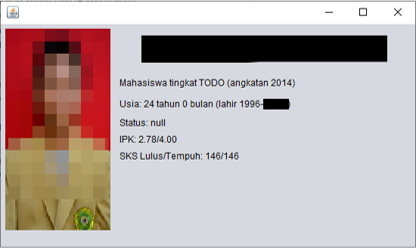
\includegraphics{prototype.png}
        	\caption{Purwarupa(\textit{Prototype})} 
        	\label{purwarupa}
        \end{figure}
        
        \begin{figure}[H]
        	\centering
        	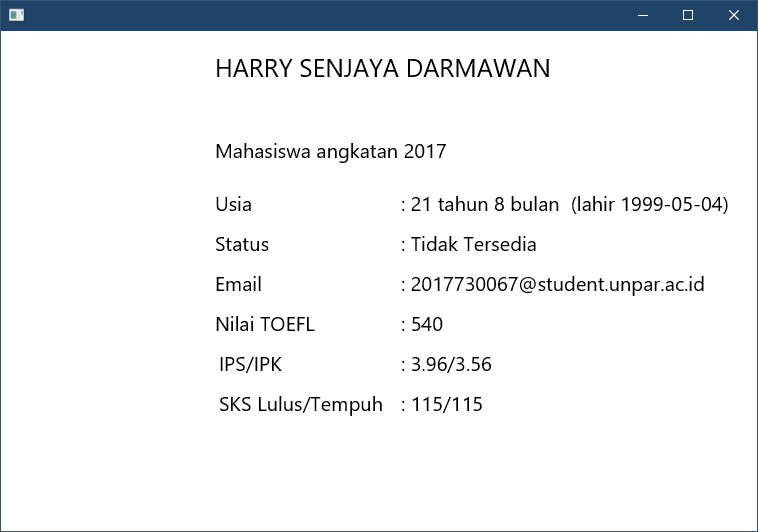
\includegraphics[scale=0.6]{UI.png}
        	\caption{Antarmuka Aplikasi} 
        	\label{ui}
        \end{figure}
        
        
        \item \textbf{Melakukan studi mengenai cara mengonversi aplikasi menjadi \textit{screen saver}}\\
		{\bf Status :} Ada sejak rencana kerja skripsi.\\
		{\bf Hasil :}  Akan dilakukan pada skripsi 2.
        
		
		\item \textbf{Mengonversi aplikasi menjadi screen saver dengan menggunakan kelas JFrame}\\
		{\bf Status :} Ada sejak rencana kerja skripsi.\\
		{\bf Hasil :} Akan dilakukan pada skripsi 2.
		
		
		\item \textbf{Melakukan pengujian dan eksperimen}\\
		{\bf Status :} Ada sejak rencana kerja skripsi.\\
		{\bf Hasil :} Akan dilakukan pada skripsi 2.
		
		
		\item \textbf{Menulis dokumen skripsi}\\
		{\bf Status :} Ada sejak rencana kerja skripsi.\\
		{\bf Hasil :} Dokumen skripsi telah dikerjakan hingga Bab 3. Bab 1 telah selesai ditulis, Bab 2 sudah ditulis sekitar 80\%, dikarenakan perlu menunggu aplikasi selesai dibuat terlebih dahulu. Bab 3 sudah menulis Analisis Pemanfaatan Jsoup.
		
	\end{enumerate}


\section{Pencapaian Rencana Kerja}
Langkah-langkah kerja yang berhasil diselesaikan dalam Skripsi 1 ini adalah sebagai berikut:
\begin{enumerate}
\item Mempelajari teknik \textit{web scraping}.
\item Menganalisis IF Student Portal dan Portal Akademik Mahasiswa.
\item Mempelajari struktur kelas SIAModels.
\item Mengimplementasikan teknik \textit{web scraping} untuk mengambil data mahasiswa.
\item Mendesain antarmuka aplikasi.
\end{enumerate}



% \section{Kendala yang Dihadapi}
% %TULISKAN BAGIAN INI JIKA DOKUMEN ANDA TIPE A ATAU C
% Kendala - kendala yang dihadapi selama mengerjakan skripsi :
% \begin{itemize}
% 	\item Terlalu banyak melakukan prokratinasi
% 	\item Terlalu banyak godaan berupa hiburan (game, film, dll)
% 	\item Skripsi diambil bersamaan dengan kuliah ASD karena selama 5 semester pertama kuliah tersebut sangat dihindari dan tidak diambil, dan selama 4 semester terakhir kuliah tersebut selalu mendapat nilai E
% 	\item Mengalami kesulitan pada saat sudah mulai membuat program komputer karena selama ini selalu dibantu teman
% \end{itemize}

\vspace{1cm}
\centering Bandung, \tanggal\\
\vspace{2cm} \nama \\ 
\vspace{1cm}

Menyetujui, \\
\ifdefstring{\jumpemb}{2}{
\vspace{1.5cm}
\begin{centering} Menyetujui,\\ \end{centering} \vspace{0.75cm}
\begin{minipage}[b]{0.45\linewidth}
% \centering Bandung, \makebox[0.5cm]{\hrulefill}/\makebox[0.5cm]{\hrulefill}/2013 \\
\vspace{2cm} Nama: \pembA \\ Pembimbing Utama
\end{minipage} \hspace{0.5cm}
\begin{minipage}[b]{0.45\linewidth}
% \centering Bandung, \makebox[0.5cm]{\hrulefill}/\makebox[0.5cm]{\hrulefill}/2013\\
\vspace{2cm} Nama: \pembB \\ Pembimbing Pendamping
\end{minipage}
\vspace{0.5cm}
}{
% \centering Bandung, \makebox[0.5cm]{\hrulefill}/\makebox[0.5cm]{\hrulefill}/2013\\
\vspace{2cm} Nama: \pembA \\ Pembimbing Tunggal
}
\end{document}

